\documentclass[border=4pt]{standalone}
\usepackage{mathptmx}
\usepackage{tikz}
\usetikzlibrary{positioning,arrows.meta,fit,calc,backgrounds}
\begin{document}
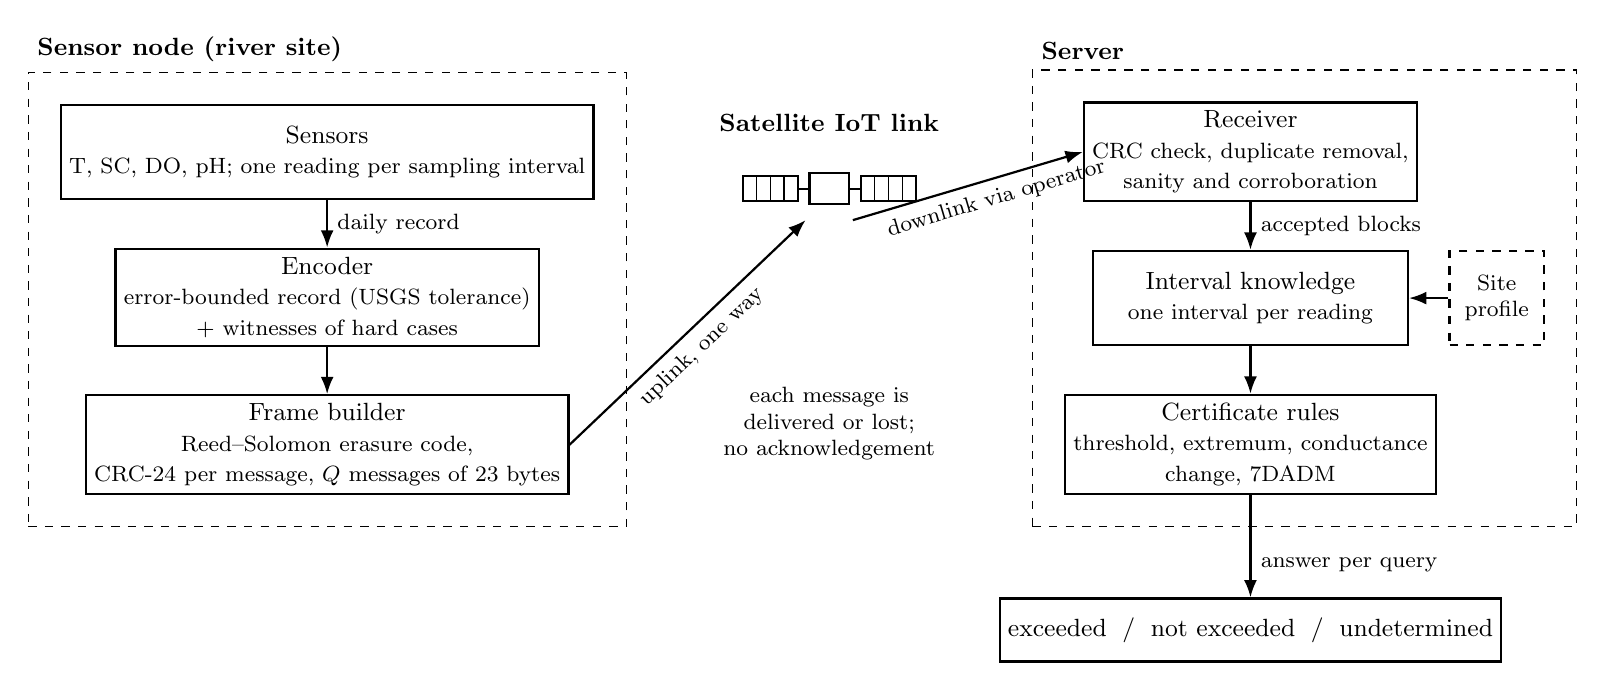
\begin{tikzpicture}[font=\small, node distance=6mm,
  comp/.style={draw, thick, align=center, minimum width=40mm, minimum height=12mm, fill=white, inner sep=3pt},
  tier/.style={draw, dashed, inner sep=4mm},
  ttl/.style={font=\small\bfseries, anchor=south west},
  arr/.style={-{Latex[length=2.2mm]}, thick},
  note/.style={font=\footnotesize, align=left}]

  % ---------------- tier 1: sensor node at the river site
  \node[comp] (sens) {Sensors\\{\footnotesize T, SC, DO, pH; one reading per sampling interval}};
  \node[comp, below=of sens] (enc) {Encoder\\{\footnotesize error-bounded record (USGS tolerance)}\\{\footnotesize + witnesses of hard cases}};
  \node[comp, below=of enc] (frm) {Frame builder\\{\footnotesize Reed--Solomon erasure code,}\\{\footnotesize CRC-24 per message, $Q$ messages of 23 bytes}};
  \draw[arr] (sens) -- node[right, note] {daily record} (enc);
  \draw[arr] (enc) -- (frm);
  \node[tier, fit=(sens)(enc)(frm)] (t1) {};
  \node[ttl] at (t1.north west) {Sensor node (river site)};

  % ---------------- tier 3: server
  \node[comp, right=62mm of sens] (rx) {Receiver\\{\footnotesize CRC check, duplicate removal,}\\{\footnotesize sanity and corroboration}};
  \node[comp, below=of rx] (know) {Interval knowledge\\{\footnotesize one interval per reading}};
  \node[comp, below=of know] (cert) {Certificate rules\\{\footnotesize threshold, extremum, conductance}\\{\footnotesize change, 7DADM}};
  \draw[arr] (rx) -- node[right, note] {accepted blocks} (know);
  \draw[arr] (know) -- (cert);
  \node[comp, dashed, right=5mm of know, minimum width=12mm, font=\footnotesize] (prof) {Site\\profile};
  \draw[arr] (prof) -- (know);
  \node[tier, fit=(rx)(know)(cert)(prof)] (t3) {};
  \node[ttl] at (t3.north west) {Server};
  \node[comp, below=13mm of cert, minimum height=8mm] (out) {exceeded \;/\; not exceeded \;/\; undetermined};

  % ---------------- tier 2: one-way satellite link
  \coordinate (sat) at ($(t1.east)!0.5!(t3.west)+(0,14mm)$);
  \begin{scope}[shift={(sat)}, thick]
    \draw[fill=white] (-2.5mm,-2mm) rectangle (2.5mm,2mm);
    \draw (-11mm,-1.6mm) rectangle (-4mm,1.6mm); \draw (4mm,-1.6mm) rectangle (11mm,1.6mm);
    \foreach \x in {-9.25,-7.5,-5.75} \draw[thin] (\x mm,-1.6mm) -- (\x mm,1.6mm);
    \foreach \x in {5.75,7.5,9.25} \draw[thin] (\x mm,-1.6mm) -- (\x mm,1.6mm);
    \draw (-4mm,0) -- (-2.5mm,0); \draw (2.5mm,0) -- (4mm,0);
  \end{scope}
  \node[font=\small\bfseries, above=6mm of sat] {Satellite IoT link};
  \draw[arr] (frm.east) -- ($(sat)+(-3mm,-4mm)$) node[pos=0.5, sloped, below, note] {uplink, one way};
  \draw[arr] ($(sat)+(3mm,-4mm)$) -- (rx.west) node[pos=0.6, sloped, below, note] {downlink via operator};
  \node[note, align=center, below=24mm of sat] {each message is\\delivered or lost;\\no acknowledgement};
  \draw[arr] (cert) -- node[pos=0.68, right, note] {answer per query} (out);
\end{tikzpicture}
\end{document}
